\documentclass[11pt]{article}

% --- Geometry and basic packages ---
\usepackage[margin=1in]{geometry}
\usepackage{amsmath,amssymb,amsthm}
\usepackage{physics}
\usepackage{slashed}
\usepackage{bm}
\usepackage{xcolor}
\usepackage[most]{tcolorbox}
\usepackage{tikz}
\usetikzlibrary{decorations.markings,arrows.meta,positioning,calc}
\usepackage{hyperref}
\hypersetup{colorlinks=true,linkcolor=blue!50!black,citecolor=blue!50!black}
\usepackage{enumitem}
\usepackage{fancyhdr}
\usepackage{parskip}

% --- Header / footer ---
\pagestyle{fancy}
\fancyhf{}
\rhead{\small PHYS 7502 --- H2 Electroweak Mixing}
\lhead{\small Parker}
\cfoot{\thepage}

% --- Color-coded tcolorbox environments ---
\newtcolorbox{problembox}[1][]{enhanced,colback=violet!5,colframe=violet!70!black,
  fonttitle=\bfseries,title=Problem Statement,#1}
\newtcolorbox{deliverbox}[1][]{enhanced,colback=orange!5,colframe=orange!70!black,
  fonttitle=\bfseries,title=Deliverables,#1}
\newtcolorbox{conceptbox}[1][]{enhanced,colback=blue!5,colframe=blue!70!black,
  fonttitle=\bfseries,title=Concept / Definition,#1}
\newtcolorbox{termbox}[1][]{enhanced,colback=violet!4,colframe=violet!50!black,
  fonttitle=\bfseries,title=Term Refresher,#1}
\newtcolorbox{resultbox}[1][]{enhanced,colback=red!5,colframe=red!70!black,
  fonttitle=\bfseries,title=Key Result,#1}
\newtcolorbox{insightbox}[1][]{enhanced,colback=green!5,colframe=green!50!black,
  fonttitle=\bfseries,title=Physical Insight,#1}
\newtcolorbox{intuitionbox}[1][]{enhanced,colback=yellow!10,colframe=yellow!50!black,
  fonttitle=\bfseries,title=Intuition,#1}
\newtcolorbox{warnbox}[1][]{enhanced,colback=gray!10,colframe=gray!60!black,
  fonttitle=\bfseries,title=Warning / Convention Pitfall,#1}
\newtcolorbox{strategybox}[1][]{enhanced,colback=cyan!4,colframe=cyan!60!black,
  fonttitle=\bfseries,title=Strategy,#1}
\newtcolorbox{contextbox}[1][]{enhanced,colback=blue!3,colframe=blue!50!black,
  fonttitle=\bfseries,title=Background \& References,#1}
\newtcolorbox{stepbox}[1][]{enhanced,colback=cyan!2,colframe=cyan!50!black,
  fonttitle=\bfseries,title=Step,#1}

% --- Title ---
\title{\bfseries Problem H2: Electroweak Mixing of $W^{(1,2,3)}$ and $B$ \\[2pt]
       \large Glashow--Salam--Weinberg Unification}
\author{Parker --- PHYS 7502}
\date{\today}

\begin{document}
\maketitle

% =====================================================================
% RESTATEMENT
% =====================================================================
\begin{problembox}
\textbf{H2.} Give the relation that describes the ``mixing'' of the ``fundamental''
$W_0$ (this means the $\{W_1,W_2,W_3\}$ vector boson triplet) and $B$ vector bosons
of the electroweak theory, which get transformed in terms of the weak mixing angle
into the usual 4 electroweak bosons we observe ($W^+, W^-, Z^0, \gamma$).

(This is related to the ``Electroweak Unification'' part of Griffiths.)
\end{problembox}

\begin{deliverbox}
\begin{enumerate}[leftmargin=*]
  \item State the gauge group whose structure produces the four ``fundamental'' bosons
        $\{W_1, W_2, W_3, B\}$.
  \item Give the relation between the charged physical bosons $W^{\pm}_\mu$ and the
        $W^{(1,2)}_\mu$ triplet members.
  \item Give the rotation relation between the neutral physical bosons $\{A_\mu,Z_\mu\}$
        and the neutral fundamental bosons $\{W^{(3)}_\mu, B_\mu\}$, expressed in terms
        of the weak mixing (Weinberg) angle $\theta_W$.
  \item Give the definition of $\theta_W$ in terms of the two underlying gauge couplings
        $g_W$ and $g'$, and the consistency relation between $g_W$, $g'$, and the
        electromagnetic coupling $g_e$.
  \item Briefly explain \emph{why} the mixing happens (electroweak symmetry breaking).
\end{enumerate}
\end{deliverbox}

\begin{contextbox}
\textbf{Primary references for this problem.}
\begin{itemize}[leftmargin=*]
  \item \textbf{Griffiths} (2nd ed.), \emph{Introduction to Elementary Particles},
        \textbf{Ch.~9 ``Weak Interactions''}, specifically:
        \begin{itemize}[leftmargin=*]
          \item §9.6 ``Neutral Weak Interactions''
          \item §9.7 ``Electroweak Unification''
                \begin{itemize}
                  \item §9.7.1 ``Chiral Fermion States''
                  \item §9.7.2 ``Weak Isospin and Hypercharge''
                  \item §9.7.3 ``Electroweak Mixing'' \;{\small$\leftarrow$ this is the section}
                \end{itemize}
        \end{itemize}
        Key equations: \textbf{Eq.~9.148} ($W^\pm$ definition), \textbf{Eq.~9.151} (the neutral mixing matrix),
        \textbf{Eq.~9.154} (the coupling consistency relation).
  \item \textbf{Thomson}, \emph{Modern Particle Physics}, Ch.~15 ``Electroweak Unification''
        (§15.2--15.3); Eqs.~15.12, 15.17--15.18, 15.30.
  \item \textbf{Halzen \& Martin}, \emph{Quarks and Leptons}, Ch.~13 (Gauge Symmetries) and
        Ch.~14--15 (The Weinberg--Salam Model).
  \item \textbf{Mann}, \emph{An Introduction to Particle Physics and the Standard Model},
        Ch.~22 (Electroweak Unification), Ch.~23 (Electroweak Symmetry Breaking).
  \item \textbf{Lancaster \& Blundell}, \emph{QFT for the Gifted Amateur}, Ch.~47
        (The Weinberg--Salam Model).
\end{itemize}
\textbf{Convention note.} Griffiths conventions take priority. Mann uses opposite signs in two
places (the $W^\pm$ definition and the inverse rotation direction) --- these are flagged when
they appear.
\end{contextbox}

\begin{intuitionbox}
\textbf{Roadmap for this problem.} The question asks for a single relation but it has more
moving parts than it looks. Here's the path we'll take in five parts:
\begin{itemize}[leftmargin=*]
  \item \textbf{Part 1.} Where do the four ``fundamental'' bosons $\{W^1, W^2, W^3, B\}$ even
        come from? (Answer: they are the gauge fields of $SU(2)_L \otimes U(1)_Y$.)
  \item \textbf{Part 2.} How do $W^1$ and $W^2$ combine into the charged $W^\pm$? (Pure
        $SU(2)$ structure; \emph{no} mixing angle yet.)
  \item \textbf{Part 3.} How do $W^3$ and $B$ rotate into $\gamma$ and $Z$? (\emph{This}
        is where $\theta_W$ enters --- it's the heart of the question.)
  \item \textbf{Part 4.} What fixes the value of $\theta_W$? (Demanding that one of the
        rotated states is the QED photon.)
  \item \textbf{Part 5.} \emph{Why} does the rotation happen at all? (Higgs mechanism breaks
        $SU(2)_L \otimes U(1)_Y \to U(1)_{\rm em}$.)
\end{itemize}
Each part has a strategy section, slow step-by-step derivation, and explicit physical
intuition.
\end{intuitionbox}

\newpage

% =====================================================================
% PART 1 — Background and gauge group
% =====================================================================
\section*{Part 1 \,---\, Where do $W^{1,2,3}_\mu$ and $B_\mu$ come from?}

\begin{problembox}
\textbf{Restatement.} Before we can ``mix'' anything, we have to know where the four
fundamental bosons live. This part identifies the gauge group whose generators \emph{produce}
these four gauge fields, and specifies what charge each field couples to.
\end{problembox}

\begin{deliverbox}
\begin{enumerate}[leftmargin=*]
  \item Name the gauge group of the electroweak interaction and explain the meaning of
        each factor.
  \item Show that this group structure forces \emph{exactly four} gauge bosons.
  \item Identify which boson couples to which conserved charge.
  \item State the Gell-Mann--Nishijima relation $Q = T^{(3)} + Y/2$, since it underlies
        \emph{everything} in the rest of the problem.
\end{enumerate}
\end{deliverbox}

\begin{strategybox}
There are several ways to motivate the gauge group. The cleanest pedagogical path is:
\begin{itemize}[leftmargin=*]
  \item \textbf{Approach A (analogy with QED, the slow safe path):} Recall how QED is built
        as a $U(1)$ gauge theory --- one symmetry, one gauge boson, one charge. Then
        \emph{enlarge} the symmetry to capture the experimentally-observed weak interaction
        structure.
  \item \textbf{Approach B (counting generators, the quick path):} Note that $SU(N)$ has
        $N^2-1$ generators and $U(1)$ has $1$. Pick the smallest non-trivial group that
        gives more than one boson and contains a piece that survives as $U(1)_{\rm em}$.
  \item \textbf{Approach C (empirical, the physical path):} List the experimental facts the
        theory must explain (V-A charged currents, neutral currents, parity violation,
        massless photon, two heavy weak bosons). Show that $SU(2)_L \otimes U(1)_Y$ is the
        minimal symmetry consistent with all of them.
\end{itemize}
We'll do Approach A in detail and weave in pieces of B and C as we go.
\end{strategybox}

% --------- subsections of Part 1 ----------
\subsection*{1.1 \,---\, Refresher: how does QED arise as a gauge theory?}

\begin{termbox}
\textbf{Gauge symmetry.} A symmetry where the transformation parameter is allowed to depend
on spacetime: $\psi(x) \to e^{i\alpha(x)} \psi(x)$. Demanding the Lagrangian be invariant
under this \emph{forces} you to introduce a gauge field $A_\mu$ that transforms as
$A_\mu \to A_\mu - \tfrac{1}{q}\partial_\mu \alpha(x)$, and the Lagrangian must use the
covariant derivative $D_\mu = \partial_\mu + iq A_\mu$ instead of $\partial_\mu$.
The number of gauge fields equals the number of independent gauge parameters --- which is
the number of \emph{generators} of the symmetry group.

\textbf{Generator.} The Hermitian operator $T$ such that $U = e^{i \alpha T}$ is a group
element. For a Lie group of dimension $d$, there are $d$ independent generators.

\textbf{Counting rule.} For a compact Lie group $G$, the number of gauge bosons equals
$\dim(G)$:
\begin{itemize}[leftmargin=*]
  \item $U(1)$: $\dim = 1$, gives 1 boson (the photon, in QED).
  \item $SU(N)$: $\dim = N^2-1$. So $SU(2)$ gives 3 bosons, $SU(3)$ gives 8, etc.
  \item For a product group $G_1 \otimes G_2$: number of bosons is $\dim(G_1) + \dim(G_2)$.
\end{itemize}
\end{termbox}

\textbf{QED as the prototype.} QED is built on the gauge group $U(1)_{\rm em}$. The local
phase rotation $\psi(x) \to e^{i Q \alpha(x)} \psi(x)$ (where $Q$ is the electric charge of
$\psi$) is the symmetry. There is \emph{one} generator (the charge $Q$), so there is
\emph{one} gauge boson: the photon $A_\mu$. Its coupling strength is $g_e$ (the unit
electric charge), and the QED interaction Lagrangian is
\begin{equation}
\mathcal{L}_{\rm QED}^{\rm int} \;=\; -\,g_e\, j^{\rm em}_\mu A^\mu,
\qquad
j^{\rm em}_\mu \;=\; \sum_f Q_f \,\bar\psi_f \gamma_\mu \psi_f .
\end{equation}
This is the template we want to generalize.

\subsection*{1.2 \,---\, Empirical clues that point to $SU(2)_L \otimes U(1)_Y$}

\begin{insightbox}
What did experimentalists \emph{know} about the weak interaction by the early 1960s, before
GWS? Five facts:
\begin{enumerate}[leftmargin=*]
  \item The charged-current weak interaction has a $V-A$ (vector minus axial-vector) structure:
        it couples \emph{only} to left-handed fermions and right-handed antifermions.
        (Wu's $\,^{60}$Co experiment, 1957.)
  \item Charged weak currents are mediated by some massive charged boson(s) (mass scale set
        by the Fermi constant $G_F$).
  \item The known fundamental fermions sit naturally in pairs --- the doublets
        $\binom{\nu_e}{e^-}_L$, $\binom{u}{d}_L$, etc.
  \item The photon is massless, parity-conserving, and couples to electric charge.
  \item There must (probably) also be a neutral-current weak interaction, whose existence
        was \emph{predicted} by GWS and confirmed at Gargamelle in 1973.
\end{enumerate}
Items (1), (3) point to a chiral $SU(2)$ that acts only on left-handed doublets ---
\textbf{this is $\bm{SU(2)_L}$}. Item (4) demands a separate $U(1)$ with a charge that
\emph{survives} as electric charge after symmetry breaking --- this is what becomes
$U(1)_{\rm em}$, but \emph{before} symmetry breaking it is the larger $\bm{U(1)_Y}$ of weak
hypercharge. The minimal gauge group consistent with all five facts is therefore
$SU(2)_L \otimes U(1)_Y$.
\end{insightbox}

\begin{conceptbox}
\textbf{The electroweak gauge group.}
\[
\boxed{\;G_{\rm EW} \;=\; SU(2)_L \;\otimes\; U(1)_Y\;}
\]
The subscripts mean:
\begin{itemize}[leftmargin=*]
  \item ``$L$'' on $SU(2)_L$: this group acts only on \emph{left-handed} fermion doublets.
        Right-handed fermions are $SU(2)_L$ singlets and don't feel it. This is what
        encodes V-A / parity violation right into the structure of the gauge group.
  \item ``$Y$'' on $U(1)_Y$: this is \emph{not} the QED $U(1)_{\rm em}$. It is the
        $U(1)$ of \emph{weak hypercharge} $Y$. Both chiralities feel it (it's not chiral),
        but with different $Y$ values for left- and right-handed fields.
  \item The $\otimes$ is a direct product: the two factors commute, are independent, and
        \emph{neither} is contained in the other.
\end{itemize}
\end{conceptbox}

\subsection*{1.3 \,---\, Counting the gauge bosons}

\begin{stepbox}
\textbf{Count generators of each factor:}
\begin{itemize}[leftmargin=*]
  \item $SU(2)_L$: $\dim = 2^2 - 1 = 3$. Three generators
        $T^a = \tfrac{1}{2}\sigma^a$ ($a = 1, 2, 3$) where $\sigma^a$ are the Pauli
        matrices acting on the left-handed weak-isospin doublet.
        $\Rightarrow$ \textbf{three gauge fields} $W^1_\mu,\, W^2_\mu,\, W^3_\mu$,
        all with the \emph{same} coupling $g_W$ (universality is forced by non-Abelian gauge
        invariance).
  \item $U(1)_Y$: $\dim = 1$. One generator (the hypercharge operator $Y$).
        $\Rightarrow$ \textbf{one gauge field} $B_\mu$, with coupling $g'$ (Griffiths
        notation; sometimes written $g_Y$).
\end{itemize}
Total: $3 + 1 = \boxed{4 \text{ fundamental gauge bosons}}$. This matches the four physical
bosons $\{W^+, W^-, Z^0, \gamma\}$, as required.
\end{stepbox}

\begin{intuitionbox}
\textbf{Why universality?} In QED you can scale the photon coupling by hand: pick any $g_e$
you like for each species of fermion (electrons, muons, quarks). In a non-Abelian gauge
theory like $SU(2)_L$, that freedom is gone --- the structure constants $\epsilon^{abc}$ in
the commutator $[T^a, T^b] = i\epsilon^{abc} T^c$ \emph{tie} the three couplings together.
All three of $W^1, W^2, W^3$ couple with the same strength $g_W$.

The $U(1)_Y$ coupling $g'$ is independent of $g_W$ because the two factor groups don't talk
to each other. This is exactly why we end up with two free coupling constants in the
electroweak Lagrangian --- and why $\theta_W \equiv \arctan(g'/g_W)$ is non-trivial.
\end{intuitionbox}

\subsection*{1.4 \,---\, What does each boson couple to?}

\begin{conceptbox}
The interaction Lagrangian for the fermion sector is
\begin{equation}
\mathcal{L}_{\rm int} \;=\; -\, g_W \,\vec{j}_\mu \cdot \vec{W}^\mu \;-\; \tfrac{g'}{2}\, j^Y_\mu B^\mu ,
\label{eq:Lint}
\end{equation}
where:
\begin{itemize}[leftmargin=*]
  \item $\vec{j}_\mu = (j^1_\mu, j^2_\mu, j^3_\mu)$ is the \textbf{weak isospin current},
        an $SU(2)$ vector built from $\bar\chi_L \gamma_\mu T^a \chi_L$, where $\chi_L$ is a
        left-handed doublet. This couples to the triplet $\vec{W}_\mu$.
  \item $j^Y_\mu = \sum_f Y_f \,\bar\psi_f \gamma_\mu \psi_f$ is the \textbf{weak hypercharge
        current}, a singlet, summed over both chiralities (with potentially different $Y$
        for left- and right-handed components). This couples to $B_\mu$.
  \item The factor of $\tfrac{1}{2}$ in front of $g'$ is purely a Griffiths convention ---
        it's there so that hypercharge enters the covariant derivative as $Y/2$, matching
        the ``half'' on $T^a = \sigma^a/2$. Other authors absorb the $\tfrac{1}{2}$ into the
        definition of $g'$.
\end{itemize}
\end{conceptbox}

\subsection*{1.5 \,---\, The Gell-Mann--Nishijima relation (the bridge to QED)}

\begin{resultbox}
\textbf{The Gell-Mann--Nishijima relation:}
\[
\boxed{\;\;
Q \;=\; T^{(3)} \;+\; \tfrac{1}{2}\, Y
\;\;}
\]
where $Q$ is electric charge, $T^{(3)}$ is the third component of weak isospin, and $Y$ is
weak hypercharge. This relation is \emph{the} reason the electroweak theory ``contains'' QED.
\end{resultbox}

\begin{insightbox}
The Gell-Mann--Nishijima relation tells us that the electric charge $Q$ is a \emph{linear
combination} of the diagonal $SU(2)_L$ generator ($T^{(3)}$) and the $U(1)_Y$ generator ($Y$).
Consequence: the gauge boson that couples to $Q$ (the photon) must be a \emph{linear
combination} of the gauge boson that couples to $T^{(3)}$ (which is $W^3_\mu$) and the
gauge boson that couples to $Y$ (which is $B_\mu$). \textbf{The mixing in this problem is
already built into the Gell-Mann--Nishijima formula.}
\end{insightbox}

% Visual summary
\begin{center}
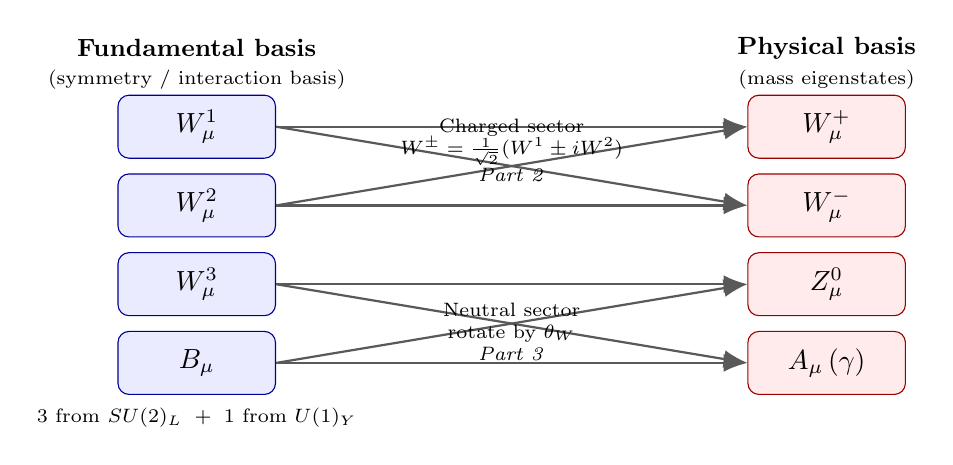
\begin{tikzpicture}[node distance=1.6cm,
  fundbox/.style={draw=blue!60!black, fill=blue!8, rounded corners,
                  minimum width=2cm, minimum height=0.8cm},
  physbox/.style={draw=red!60!black, fill=red!8, rounded corners,
                  minimum width=2cm, minimum height=0.8cm},
  arr/.style={-{Latex[length=3mm]}, thick, gray!70!black}]

  \node at (0,4) [font=\small]   {\bfseries Fundamental basis};
  \node at (0,3.6)[font=\scriptsize]{(symmetry / interaction basis)};
  \node[fundbox] (W1) at (0,3) {$W^1_\mu$};
  \node[fundbox] (W2) at (0,2) {$W^2_\mu$};
  \node[fundbox] (W3) at (0,1) {$W^3_\mu$};
  \node[fundbox] (B)  at (0,0) {$B_\mu$};
  \node[font=\scriptsize] at (0,-0.7) {3 from $SU(2)_L$\;\;+\;\;1 from $U(1)_Y$};

  \node at (8,4)  [font=\small]    {\bfseries Physical basis};
  \node at (8,3.6)[font=\scriptsize]{(mass eigenstates)};
  \node[physbox] (Wp) at (8,3) {$W^+_\mu$};
  \node[physbox] (Wm) at (8,2) {$W^-_\mu$};
  \node[physbox] (Z)  at (8,1) {$Z^0_\mu$};
  \node[physbox] (A)  at (8,0) {$A_\mu\,(\gamma)$};

  % charged sector mixing
  \draw[arr] (W1.east) -- (Wp.west);
  \draw[arr] (W2.east) -- (Wp.west);
  \draw[arr] (W1.east) -- (Wm.west);
  \draw[arr] (W2.east) -- (Wm.west);
  \node[font=\scriptsize, align=center] at (4,2.7)
       {Charged sector\\ $W^\pm = \tfrac{1}{\sqrt2}(W^1 \pm i W^2)$\\ \emph{Part 2}};

  % neutral sector mixing
  \draw[arr] (W3.east) -- (Z.west);
  \draw[arr] (B.east)  -- (Z.west);
  \draw[arr] (W3.east) -- (A.west);
  \draw[arr] (B.east)  -- (A.west);
  \node[font=\scriptsize, align=center] at (4,0.4)
       {Neutral sector\\ rotate by $\theta_W$\\ \emph{Part 3}};
\end{tikzpicture}
\end{center}

\begin{resultbox}
\textbf{Part 1 summary.} The electroweak gauge group $SU(2)_L \otimes U(1)_Y$ forces four
gauge fields:
\begin{itemize}[leftmargin=*]
  \item Three from $SU(2)_L$: $W^1_\mu, W^2_\mu, W^3_\mu$, all with coupling $g_W$,
        coupling to weak isospin currents $j^a_\mu$.
  \item One from $U(1)_Y$: $B_\mu$ with coupling $g'$, coupling to weak hypercharge
        current $j^Y_\mu$.
\end{itemize}
The Gell-Mann--Nishijima relation $Q = T^{(3)} + Y/2$ guarantees that some linear
combination of $W^3$ and $B$ couples to electric charge --- i.e., that the photon is a
mixture, not a pure $W^3$ or pure $B$. Finding that linear combination is what Parts 3--4
do.
\end{resultbox}

\newpage

% =====================================================================
% PART 2 — Charged sector
% =====================================================================
\section*{Part 2 \,---\, Charged sector: $W^{(1,2)} \to W^{\pm}$}

\begin{problembox}
\textbf{Restatement.} Express the physical \emph{charged} bosons $W^+_\mu$ and $W^-_\mu$ as
linear combinations of $W^1_\mu$ and $W^2_\mu$. This part does \emph{not} involve the
weak mixing angle --- it's pure $SU(2)$ algebra.
\end{problembox}

\begin{deliverbox}
\begin{enumerate}[leftmargin=*]
  \item Explain why $W^+$ and $W^-$ \emph{must} be complex fields (not real ones).
  \item Derive the Griffiths convention $W^\pm_\mu = \tfrac{1}{\sqrt2}(W^1_\mu \pm i W^2_\mu)$,
        including where the $\tfrac{1}{\sqrt2}$ comes from.
  \item Show that this gives back the $V-A$ vertex factor $-i\,(g_W/\sqrt2)\,\gamma^\mu \tfrac{1}{2}(1-\gamma^5)$
        we already know.
\end{enumerate}
\end{deliverbox}

\subsection*{2.1 \,---\, Why the charged sector mixes (a physical argument)}

\begin{stepbox}[title=Step 2.1: Two real fields cannot represent a charged particle]
A real-valued classical field $\phi(x) = \phi^*(x)$ corresponds, upon quantization, to a
\emph{neutral} particle that is its own antiparticle (like the $\pi^0$ or the photon). A
\emph{complex} field $\phi(x) \neq \phi^*(x)$ corresponds to a \emph{charged} particle whose
antiparticle is distinct (like the $\pi^\pm$).

The fields $W^1_\mu$ and $W^2_\mu$ are both real (they're the components of an $SU(2)$
gauge connection in the standard hermitian basis). So neither one alone can describe
$W^+$ (which has $Q = +1$) or $W^-$ (which has $Q = -1$). We need to combine them into
a \emph{complex} field whose conjugate is the antiparticle field.
\end{stepbox}

\begin{intuitionbox}
This is exactly the same trick that turns two real Klein-Gordon fields into one charged
Klein-Gordon field. If $\phi_1, \phi_2$ are real with the same mass, then
$\phi \equiv \tfrac{1}{\sqrt2}(\phi_1 + i\phi_2)$ and $\phi^* \equiv \tfrac{1}{\sqrt2}(\phi_1 - i\phi_2)$
are a charge-conjugate pair. This trick is so generic that it has nothing to do with the
weak interaction per se --- it's just \emph{how you build a charged field from two neutral
ones}.
\end{intuitionbox}

\subsection*{2.2 \,---\, The $SU(2)$ raising/lowering operators}

\begin{stepbox}[title=Step 2.2: Look at how $W^1$ and $W^2$ act inside the doublet]
Inside an $SU(2)_L$ doublet $\chi_L = \binom{\nu_L}{e_L}$, the generators $T^a = \sigma^a/2$
act as
\[
T^1 = \tfrac{1}{2}\!\begin{pmatrix} 0 & 1 \\ 1 & 0 \end{pmatrix},
\quad
T^2 = \tfrac{1}{2}\!\begin{pmatrix} 0 & -i \\ i & \phantom{-}0 \end{pmatrix},
\quad
T^3 = \tfrac{1}{2}\!\begin{pmatrix} 1 & \phantom{-}0 \\ 0 & -1 \end{pmatrix}.
\]
Now the \emph{raising} and \emph{lowering} operators $T^\pm$ are defined exactly as in
ordinary angular momentum:
\[
T^\pm \;\equiv\; T^1 \pm i T^2 \;=\; \begin{pmatrix} 0 & 1 \\ 0 & 0 \end{pmatrix} \;\text{or}\; \begin{pmatrix} 0 & 0 \\ 1 & 0 \end{pmatrix}.
\]
$T^+$ takes $e_L \to \nu_L$ (raises $T^{(3)}$), and $T^-$ does the reverse.

\textbf{The physical $W^\pm$ fields are exactly the components of the gauge field that
couple to these raising/lowering operators.}
\end{stepbox}

\begin{termbox}
\textbf{Why the analogy with $J_\pm$ in angular momentum?} It's not analogy --- it's the same
mathematics. Weak isospin $\vec{T}$ obeys exactly the $SU(2)$ commutation relations
$[T^a, T^b] = i\epsilon^{abc} T^c$, just like ordinary angular momentum. The operator
$T^+$ raises $T^{(3)}$, $T^-$ lowers it. Two states in a doublet have $T^{(3)} = \pm \tfrac{1}{2}$,
exactly like a spin-$\tfrac{1}{2}$ particle. (You used this same SU(2) bridge in the
QCD/SU(3) work earlier --- the weak isospin is just the leftmost subgroup of the same
mathematical structure.)
\end{termbox}

\subsection*{2.3 \,---\, Define $W^\pm$ to make the Lagrangian clean}

\begin{stepbox}[title=Step 2.3: Combine $W^1$ and $W^2$ in the same way]
Look at the charged piece of the gauge interaction (Griffiths Eq.~9.146--9.147):
\[
\mathcal{L}_{\rm CC}
\;=\; -\,g_W\!\left( j^1_\mu W^{1\mu} + j^2_\mu W^{2\mu} \right) .
\]
We \emph{want} to write this as $-\tfrac{g_W}{\sqrt2}(j^+_\mu W^{-\mu} + j^-_\mu W^{+\mu})$.
That requires defining
\[
\boxed{\;\;
W^{\pm}_\mu \;\equiv\; \frac{1}{\sqrt{2}}\!\left( W^1_\mu \pm i\, W^2_\mu \right)
\quad\text{[\textbf{Griffiths Eq.~9.148}]}
\;\;}
\]
and the corresponding currents $j^\pm_\mu \equiv j^1_\mu \mp i j^2_\mu$.

\textbf{Verification (one line of algebra).}
\begin{align*}
j^+_\mu W^{-\mu} + j^-_\mu W^{+\mu}
&= (j^1 - i j^2)_\mu \cdot \tfrac{1}{\sqrt2}(W^1 - i W^2)^\mu
   + (j^1 + i j^2)_\mu \cdot \tfrac{1}{\sqrt2}(W^1 + i W^2)^\mu \\
&= \tfrac{1}{\sqrt2}\!\left[
   (j^1 W^{1} + j^2 W^{2}) - i(j^1 W^{2} - j^2 W^{1})
   + (j^1 W^{1} + j^2 W^{2}) + i(j^1 W^{2} - j^2 W^{1})
   \right] \\
&= \tfrac{2}{\sqrt2}(j^1_\mu W^{1\mu} + j^2_\mu W^{2\mu}) \\
&= \sqrt{2}\,(j^1_\mu W^{1\mu} + j^2_\mu W^{2\mu}).
\end{align*}
The two cross-terms $\pm i(j^1 W^2 - j^2 W^1)$ cancel exactly --- this is the whole point.
So
\[
j^1_\mu W^{1\mu} + j^2_\mu W^{2\mu}
\;=\; \tfrac{1}{\sqrt2}\!\left( j^+_\mu W^{-\mu} + j^-_\mu W^{+\mu} \right) ,
\]
and therefore
$\mathcal{L}_{\rm CC} = -\tfrac{g_W}{\sqrt2}\!\left( j^+_\mu W^{-\mu} + j^-_\mu W^{+\mu} \right)$,
which is the standard charged-current form.
\end{stepbox}

\begin{intuitionbox}
\textbf{Where does the $\tfrac{1}{\sqrt 2}$ come from?} It's just normalization. We want the
two real fields $(W^1, W^2)$ to map onto a complex field $(W^+, W^{+\,*}) = (W^+, W^-)$ such
that the kinetic term in the Lagrangian retains canonical normalization. Specifically,
$-\tfrac{1}{4}\left[(F^1_{\mu\nu})^2 + (F^2_{\mu\nu})^2\right]$ becomes $-\tfrac{1}{2} F^+_{\mu\nu} F^{-\,\mu\nu}$
when you make the substitution with the $\tfrac{1}{\sqrt2}$ factor. Drop the $\tfrac{1}{\sqrt2}$
and you'd have to write $-\tfrac{1}{2}$ in some places and $-1$ in others.
\end{intuitionbox}

\subsection*{2.4 \,---\, Recover the $V-A$ vertex factor}

\begin{stepbox}[title=Step 2.4: Check that the standard vertex factor pops out]
Consider the process $e^- \to \nu_e + W^-$ (or its crossed version). Griffiths
(Eq.~9.149) writes the relevant current as
\[
j^-_\mu \;=\; \bar{\nu}_L \gamma_\mu e_L \;=\; \bar{\nu}\, \gamma_\mu \tfrac{1}{2}(1-\gamma^5)\, e ,
\]
where the second form uses the chiral projector $P_L = \tfrac{1}{2}(1-\gamma^5)$.
Plugging into $\mathcal{L}_{\rm CC} \supset -\tfrac{g_W}{\sqrt2}\, j^-_\mu W^{+\mu}$:
\[
\mathcal{L} \;\supset\; -\,\frac{g_W}{\sqrt2}\,\bar{\nu}\, \gamma_\mu \tfrac{1}{2}(1-\gamma^5)\, e\; W^{+\mu} ,
\]
giving the vertex factor
\[
\boxed{\;\;
-\,i\,\frac{g_W}{\sqrt{2}}\, \gamma^\mu \tfrac{1}{2}(1-\gamma^5)
\quad\text{(Griffiths Eq.~9.150 / Eq.~9.5)}\;\;}
\]
which is precisely the $V-A$ vertex factor we started with way back in §9.1. Consistency
check passed.
\end{stepbox}

% --- Convention pitfall ---
\begin{warnbox}
\textbf{Sign convention pitfall (this comes up in homework grading every semester).}
Two conventions exist for the sign in front of $iW^2$:
\begin{itemize}[leftmargin=*]
  \item \textbf{Griffiths} (Eq.~9.148):
        $W^\pm_\mu = \tfrac{1}{\sqrt2}(W^1_\mu \pm i W^2_\mu)$.
  \item \textbf{Thomson} (Eq.~15.12) and \textbf{Mann} (Eq.~23.45):
        $W^\pm_\mu = \tfrac{1}{\sqrt2}(W^1_\mu \mp i W^2_\mu)$.
\end{itemize}
The two conventions differ \emph{only} in which combination is labeled ``$+$'' versus ``$-$''.
The physics is identical. But you must be consistent --- whatever sign you pick for $W^\pm$,
you must use the same sign for $T^\pm = T^1 \pm i T^2$ and $j^\pm$. \emph{Don't cross
conventions across textbooks mid-derivation.}

For Frantz's class, follow Griffiths' convention since the rest of the chapter does.
\end{warnbox}

\begin{resultbox}
\textbf{Part 2 result.}
\[
\boxed{\;\;
W^{\pm}_\mu \;=\; \frac{1}{\sqrt{2}}\!\left( W^1_\mu \pm i\, W^2_\mu \right)
\;\;}
\qquad\text{(Griffiths Eq.~9.148; charged sector mixing).}
\]
This is a unitary change of basis: two real fields $(W^1, W^2)$ get repackaged as one
complex field $W^+$ and its conjugate $W^-$. \textbf{No mixing angle, no Higgs, no
electroweak unification needed.} It's just $SU(2)$ raising/lowering structure.
\end{resultbox}

\newpage

% =====================================================================
% PART 3 — Neutral sector mixing
% =====================================================================
\section*{Part 3 \,---\, Neutral sector: $\{W^3, B\} \to \{\gamma, Z\}$}

\begin{problembox}
\textbf{Restatement.} Express the physical \emph{neutral} bosons --- the photon $A_\mu$
and the neutral weak boson $Z_\mu$ --- as linear combinations of the gauge fields $W^3_\mu$
and $B_\mu$. This is where the weak mixing angle $\theta_W$ enters, and it's the heart of
the question.
\end{problembox}

\begin{deliverbox}
\begin{enumerate}[leftmargin=*]
  \item Argue why neither $W^3$ alone nor $B$ alone can be the photon.
  \item Argue why the most general transformation between two real, neutral fields with the
        same kinetic term is an $SO(2)$ rotation (one parameter, $\theta_W$).
  \item Write down the rotation in Griffiths' convention (Eq.~9.151).
  \item Write the inverse relation $\{W^3, B\}$ in terms of $\{A, Z\}$.
\end{enumerate}
\end{deliverbox}

\subsection*{3.1 \,---\, Why $W^3 \neq \gamma$}

\begin{stepbox}[title=Step 3.1: $W^3$ couples only to left-handed fermions]
The current that $W^3$ couples to is $j^3_\mu$ from the $SU(2)_L$ algebra:
\[
j^3_\mu \;=\; g_W\, \bar\chi_L \gamma_\mu T^{(3)} \chi_L
\;=\; \tfrac{1}{2} g_W\!\left( \bar\nu_L \gamma_\mu \nu_L - \bar e_L \gamma_\mu e_L \right) .
\]
Notice everything here is left-handed (subscript $L$). Right-handed fermions are $SU(2)_L$
singlets and don't appear. \textbf{So $W^3$ couples to LH fermions only --- it is maximally
parity-violating.}

The photon, on the other hand, couples to electric charge $Q$, which is parity-conserving
(QED preserves parity). Therefore $W^3 \neq \gamma$. ✓
\end{stepbox}

\subsection*{3.2 \,---\, Why $B \neq \gamma$}

\begin{stepbox}[title=Step 3.2: $B$ couples to weak hypercharge $Y$, not to electric charge $Q$]
The current that $B$ couples to is $j^Y_\mu$, summed over both chiralities with potentially
different $Y$ values:
\[
j^Y_\mu \;=\; \sum_f Y_f\, \bar\psi_f \gamma_\mu \psi_f .
\]
For the lepton doublet, the assignments are $Y_{e_L} = Y_{\nu_L} = -1$ and $Y_{e_R} = -2$,
$Y_{\nu_R} = 0$ (Thomson §15.3 and Griffiths §9.7.2). These are \emph{not} proportional to
electric charge $Q$ (else there would be no need for a separate hypercharge). For example,
the neutrino has $Q = 0$ but $Y_{\nu_L} = -1 \neq 0$.

Therefore $B \neq \gamma$ either. ✓ \textbf{The photon must be a non-trivial linear
combination of both $W^3$ and $B$.}
\end{stepbox}

\begin{insightbox}
The two arguments together rule out the ``trivial'' identifications and force the photon
to be a real mixture. Looking at it through the Gell-Mann--Nishijima lens:
\[
Q \;=\; T^{(3)} \;+\; \tfrac{1}{2} Y \quad\Rightarrow\quad \gamma\;\text{couples to a combination of}\; T^{(3)}\;\text{and}\;Y.
\]
And since $W^3$ couples to $T^{(3)}$ and $B$ couples to $Y$, the photon must be a combination
of $W^3$ and $B$. The orthogonal combination is the $Z^0$.
\end{insightbox}

\subsection*{3.3 \,---\, The most general orthogonal mixing in 2D is a rotation}

\begin{stepbox}[title=Step 3.3: Write down the most general allowed mixing]
We have two real, neutral fields $W^3_\mu$ and $B_\mu$ with canonically-normalized kinetic
terms:
\[
\mathcal{L}_{\rm kin} \;\supset\; -\tfrac{1}{4}\,(F^{(W^3)}_{\mu\nu})^2 \;-\; \tfrac{1}{4}\,(F^{(B)}_{\mu\nu})^2 .
\]
Any change of basis $(W^3, B) \to (A, Z)$ that \emph{preserves} the canonical normalization
of the kinetic terms must be an orthogonal transformation. In 2D, the only orthogonal
transformations are
\begin{itemize}[leftmargin=*]
  \item Rotations (determinant $+1$): $\binom{A}{Z} = R(\theta) \binom{B}{W^3}$ where $R(\theta) = \binom{\cos\theta\;\;\sin\theta}{-\sin\theta\;\;\cos\theta}$.
  \item Reflections (determinant $-1$): same as a rotation followed by flipping a sign.
\end{itemize}
Reflections just amount to relabeling, so without loss of generality the mixing is a
rotation by some angle $\theta_W$:
\[
\begin{pmatrix} A_\mu \\ Z_\mu \end{pmatrix}
\;=\;
\begin{pmatrix} \cos\theta_W & \phantom{-}\sin\theta_W \\[2pt] -\sin\theta_W & \phantom{-}\cos\theta_W \end{pmatrix}
\begin{pmatrix} B_\mu \\ W^3_\mu \end{pmatrix}.
\]
Reading off rows:
\[
\boxed{\;\;
\begin{aligned}
A_\mu &= \phantom{-}B_\mu \cos\theta_W \;+\; W^3_\mu \sin\theta_W, \\[3pt]
Z_\mu &= -B_\mu \sin\theta_W \;+\; W^3_\mu \cos\theta_W
\end{aligned}
\;\;}
\quad\text{[\textbf{Griffiths Eq.~9.151}; Thomson Eqs.~15.17--15.18]}
\]
This is the central relation requested by H2.
\end{stepbox}

\begin{conceptbox}
\textbf{What ``mixing'' means here.} The fields $\{W^3, B\}$ are the gauge fields you'd write
down if you were trying to make the gauge \emph{Lagrangian} look as simple as possible
(symmetry is manifest in this basis). The fields $\{A, Z\}$ are the ones that propagate as
free particles with definite mass (mass eigenstates). These are two different orthogonal
bases of the same 2-dimensional space of neutral fields, and they're related by a single
rotation angle $\theta_W$.

This is exactly analogous to:
\begin{itemize}[leftmargin=*]
  \item Neutrino flavor states $(\nu_e, \nu_\mu)$ vs.\ mass states $(\nu_1, \nu_2)$
        --- mixing matrix is the PMNS rotation by angle $\theta_{12}$.
  \item Quark flavor states $(d, s)$ vs.\ mass states (real $d, s$ quarks)
        --- mixing matrix is the Cabibbo rotation by angle $\theta_C$.
\end{itemize}
In each case: one basis is natural for writing the interaction Lagrangian, the other is
natural for identifying physical particles. The rotation between them encodes physics; the
\emph{angle} is a measured parameter.
\end{conceptbox}

\subsection*{3.4 \,---\, The inverse relation}

Since rotations are orthogonal, $R^{-1} = R^T$. Inverting:
\begin{equation}
\begin{pmatrix} B_\mu \\ W^3_\mu \end{pmatrix}
\;=\;
\begin{pmatrix} \cos\theta_W & -\sin\theta_W \\[2pt] \sin\theta_W & \phantom{-}\cos\theta_W \end{pmatrix}
\begin{pmatrix} A_\mu \\ Z_\mu \end{pmatrix},
\qquad
\boxed{\;\;
\begin{aligned}
B_\mu &= \phantom{-}A_\mu\cos\theta_W \;-\; Z_\mu \sin\theta_W, \\
W^3_\mu &= \phantom{-}A_\mu\sin\theta_W \;+\; Z_\mu \cos\theta_W .
\end{aligned}
\;\;}
\end{equation}
We will need this inverse form in Part 4 when we substitute back into the gauge interaction
Lagrangian to determine $\theta_W$.

\begin{warnbox}
\textbf{Convention check vs. Mann.} Mann (Eq.~23.45) writes the inverse rotation in the
opposite direction, which corresponds to $\theta_W \to -\theta_W$. This is just a sign
convention --- the physical angle is the same. \textbf{Griffiths/Thomson/Halzen-Martin/Lancaster
\& Blundell all agree on the sign.} Mann is the outlier. Stick with Griffiths.
\end{warnbox}

\subsection*{3.5 \,---\, Visual: the rotation in field space}

\begin{center}
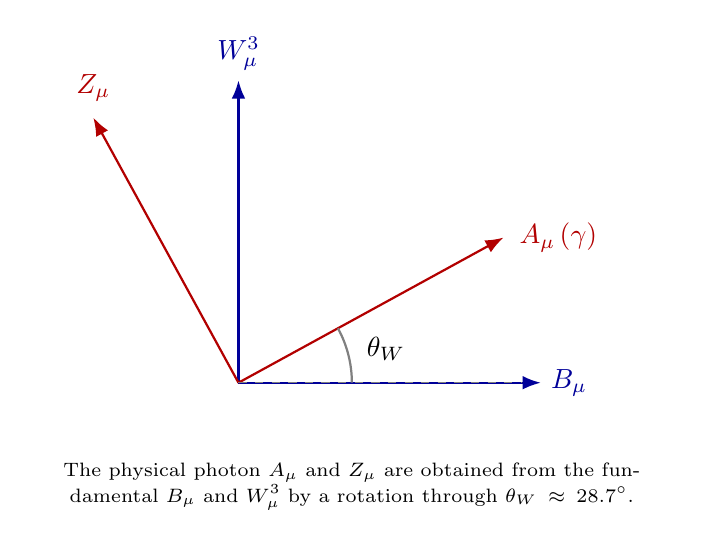
\begin{tikzpicture}[scale=2.4,>=Latex]
  % B horizontal, W3 vertical (fundamental basis, blue)
  \draw[->,thick,blue!60!black] (0,0) -- (1.6,0) node[right] {$B_\mu$};
  \draw[->,thick,blue!60!black] (0,0) -- (0,1.6) node[above] {$W^3_\mu$};
  % A and Z (physical basis, red), rotated by theta_W ≈ 28.7°
  \def\thetaW{28.7}
  \draw[->,thick,red!70!black, rotate=\thetaW] (0,0) -- (1.6,0) node[right=2pt] {$A_\mu\,(\gamma)$};
  \draw[->,thick,red!70!black, rotate=\thetaW] (0,0) -- (0,1.6) node[above=2pt] {$Z_\mu$};
  % angle arc and label
  \draw[thick,black!50!white] (0.6,0) arc (0:\thetaW:0.6);
  \node at (0.78,0.18) {$\theta_W$};
  % small dotted helper showing the rotation
  \draw[dashed,gray] (0,0) -- (1.5,0);
  \node[align=center,font=\scriptsize, text width=8cm] at (0.6,-0.55)
    {The physical photon $A_\mu$ and $Z_\mu$ are obtained from the
     fundamental $B_\mu$ and $W^3_\mu$ by a rotation through $\theta_W \approx 28.7^\circ$.};
\end{tikzpicture}
\end{center}

\begin{intuitionbox}
The picture says: \emph{the photon is mostly $B$ with a $\sin^2\theta_W \approx 23\%$
admixture of $W^3$}. Concretely, since $\sin^2\theta_W \approx 0.231$:
\begin{itemize}[leftmargin=*]
  \item $A_\mu \approx 0.88\, B_\mu + 0.48\, W^3_\mu$ \quad (the photon, massless).
  \item $Z_\mu \approx -0.48\, B_\mu + 0.88\, W^3_\mu$ \quad (the $Z^0$, $\sim 91$ GeV).
\end{itemize}
The $Z$ is the orthogonal combination --- mostly $W^3$ with a smaller $B$ component.
This is why the $Z$ couples to fermions in a more complicated way than the photon does
(it has both vector and axial-vector pieces, with strengths that depend on $\theta_W$).
\end{intuitionbox}

\begin{resultbox}
\textbf{Part 3 result --- the answer to H2.}
\[
\boxed{\;\;
\begin{aligned}
A_\mu &= \phantom{-}B_\mu \cos\theta_W \;+\; W^3_\mu \sin\theta_W \quad(=\gamma), \\[3pt]
Z_\mu &= -B_\mu \sin\theta_W \;+\; W^3_\mu \cos\theta_W .
\end{aligned}
\;\;}
\]
$\theta_W$ is a single mixing angle (the Weinberg angle), measured experimentally.
\end{resultbox}

\newpage

% =====================================================================
% PART 4 — Determining theta_W and coupling consistency
% =====================================================================
\section*{Part 4 \,---\, Determining $\theta_W$ and the unification relation}

\begin{problembox}
\textbf{Restatement.} The mixing angle $\theta_W$ is not arbitrary --- it is fixed by
demanding that one of the rotated fields ($A_\mu$) couple with strength $g_e$ to electric
charge $Q$. Show how this requirement gives Griffiths' Eq.~9.154:
$g_W \sin\theta_W = g' \cos\theta_W = g_e$, and equivalently $\tan\theta_W = g'/g_W$.
\end{problembox}

\begin{deliverbox}
\begin{enumerate}[leftmargin=*]
  \item Substitute the inverse rotation $W^3 = A \sin\theta_W + Z \cos\theta_W$ and
        $B = A \cos\theta_W - Z \sin\theta_W$ into the neutral piece of the Lagrangian.
  \item Read off the coefficient of $A_\mu$ and demand it equal $-g_e\, j^{\rm em}_\mu$.
  \item Use the Gell-Mann--Nishijima decomposition $j^{\rm em} = j^3 + \tfrac{1}{2} j^Y$ to
        match coefficients of $j^3$ and $j^Y$ separately.
  \item Out drops the consistency relation and $\tan\theta_W = g'/g_W$.
  \item Quote the experimental value of $\sin^2\theta_W$.
\end{enumerate}
\end{deliverbox}

\begin{strategybox}
The whole derivation is one substitution + one matching. The hardest part is keeping track
of the factor of $\tfrac{1}{2}$ in front of $g'$ (Griffiths' convention), which combines
with the factor of $\tfrac{1}{2}$ from the Gell-Mann--Nishijima formula $Q = T^{(3)} + \tfrac{1}{2} Y$
to give the simple form of Eq.~9.154.
\end{strategybox}

\subsection*{4.1 \,---\, Substitute the inverse rotation into the Lagrangian}

\begin{stepbox}[title=Step 4.1: Plug in $W^3$ and $B$ in terms of $A$ and $Z$]
The neutral piece of the gauge interaction Lagrangian (from Eq.~\ref{eq:Lint}) is
\[
\mathcal{L}_{\rm neut} \;=\; -\, g_W\, j^3_\mu W^{3\mu} \;-\; \tfrac{g'}{2}\, j^Y_\mu B^\mu .
\]
Substitute $W^{3\mu} = A^\mu \sin\theta_W + Z^\mu \cos\theta_W$ and
$B^\mu = A^\mu \cos\theta_W - Z^\mu \sin\theta_W$:
\begin{align}
\mathcal{L}_{\rm neut}
&= -\, g_W\, j^3_\mu \!\left( A^\mu \sin\theta_W + Z^\mu \cos\theta_W \right) \notag\\
&\qquad\;\;\; -\, \tfrac{g'}{2}\, j^Y_\mu \!\left( A^\mu \cos\theta_W - Z^\mu \sin\theta_W \right) .
\end{align}
Now collect terms separately by which physical field $A^\mu$ or $Z^\mu$ they multiply:
\begin{align}
\mathcal{L}_{\rm neut}
&= -\,A^\mu \!\left( g_W \sin\theta_W \, j^3_\mu \;+\; \tfrac{g'}{2} \cos\theta_W \, j^Y_\mu \right) \notag\\[2pt]
&\qquad\;\; -\,Z^\mu \!\left( g_W \cos\theta_W \, j^3_\mu \;-\; \tfrac{g'}{2} \sin\theta_W \, j^Y_\mu \right) .
\label{eq:rotated}
\end{align}
This is just the Lagrangian rewritten in the new basis. \emph{Nothing about electroweak
unification has been imposed yet --- this is purely algebra.}
\end{stepbox}

\subsection*{4.2 \,---\, The QED coupling sets the constraint}

\begin{stepbox}[title=Step 4.2: Demand that the photon term has QED form]
The standard QED interaction is
\[
\mathcal{L}_{\rm QED} \;=\; -\, g_e\, j^{\rm em}_\mu A^\mu ,
\qquad
j^{\rm em}_\mu \;=\; \sum_f Q_f \,\bar\psi_f \gamma_\mu \psi_f .
\]
For the electroweak theory to \emph{contain} QED at low energies, the $A_\mu$ piece in
\eqref{eq:rotated} must equal $-g_e\, j^{\rm em}_\mu A^\mu$. Therefore we demand:
\[
g_W \sin\theta_W \, j^3_\mu \;+\; \tfrac{g'}{2} \cos\theta_W \, j^Y_\mu
\;\stackrel{!}{=}\; g_e\, j^{\rm em}_\mu .
\]
\end{stepbox}

\subsection*{4.3 \,---\, Use Gell-Mann--Nishijima to match coefficients}

\begin{stepbox}[title=Step 4.3: Decompose $j^{\rm em}$ in terms of $j^3$ and $j^Y$]
The Gell-Mann--Nishijima relation $Q = T^{(3)} + \tfrac{1}{2} Y$, written at the current level
(integrate the operator equation against $\bar\psi \gamma_\mu \psi$), gives
\[
j^{\rm em}_\mu \;=\; j^3_\mu \;+\; \tfrac{1}{2}\, j^Y_\mu .
\]
So the demand becomes
\[
g_W \sin\theta_W \, j^3_\mu \;+\; \tfrac{g'}{2} \cos\theta_W \, j^Y_\mu
\;=\; g_e\!\left( j^3_\mu \;+\; \tfrac{1}{2}\, j^Y_\mu \right) .
\]
Match coefficients of $j^3_\mu$ and $j^Y_\mu$ separately (since they're independent currents):
\begin{align}
\text{[coeff. of }j^3\text{]:}\quad &\; g_W \sin\theta_W \;=\; g_e , \\[2pt]
\text{[coeff. of }j^Y\text{]:}\quad &\; \tfrac{g'}{2} \cos\theta_W \;=\; \tfrac{g_e}{2}
\quad\Longleftrightarrow\quad g' \cos\theta_W \;=\; g_e .
\end{align}
\end{stepbox}

\subsection*{4.4 \,---\, The unification consistency relation}

\begin{resultbox}
\textbf{Combining the two matching equations:}
\[
\boxed{\;\;
g_W \sin\theta_W \;=\; g' \cos\theta_W \;=\; g_e
\;\;}
\qquad\text{[\textbf{Griffiths Eq.~9.154}]}
\]
\textbf{Solve for $\theta_W$ by dividing:}
\[
\boxed{\;\;
\tan\theta_W \;=\; \frac{g'}{g_W}
\;\;}
\]
\textbf{Solve for the trig functions individually} using $\sin^2 + \cos^2 = 1$:
\[
\sin\theta_W \;=\; \frac{g'}{\sqrt{g_W^2 + g'^2}},
\qquad
\cos\theta_W \;=\; \frac{g_W}{\sqrt{g_W^2 + g'^2}},
\qquad
g_e \;=\; \frac{g_W \, g'}{\sqrt{g_W^2 + g'^2}}.
\]
\end{resultbox}

\begin{insightbox}
Take a moment to appreciate what just happened. We started with two independent gauge
couplings $g_W$ (for $SU(2)_L$) and $g'$ (for $U(1)_Y$). We rotated $W^3$ and $B$ by some
angle $\theta_W$. \textbf{Just by demanding that the resulting photon $A_\mu$ couple to
electric charge with strength $g_e$, we got two equations in two unknowns ($\theta_W$ and
the relation between $g_W, g', g_e$).} The result fixes \emph{both} the angle and a
non-trivial relation among the three couplings. This is what physicists mean when they
say the electroweak theory ``unifies'' electromagnetism and the weak force.

The theory does \emph{not} predict $\theta_W$ from first principles --- you still have to
measure either $g_W$ and $g'$ (or, equivalently, $g_e$ and $\theta_W$) from experiment. But
it predicts a \emph{relation} among them. Three couplings, two equations, one free parameter.
\end{insightbox}

\subsection*{4.5 \,---\, The geometric picture: a right triangle}

\begin{center}
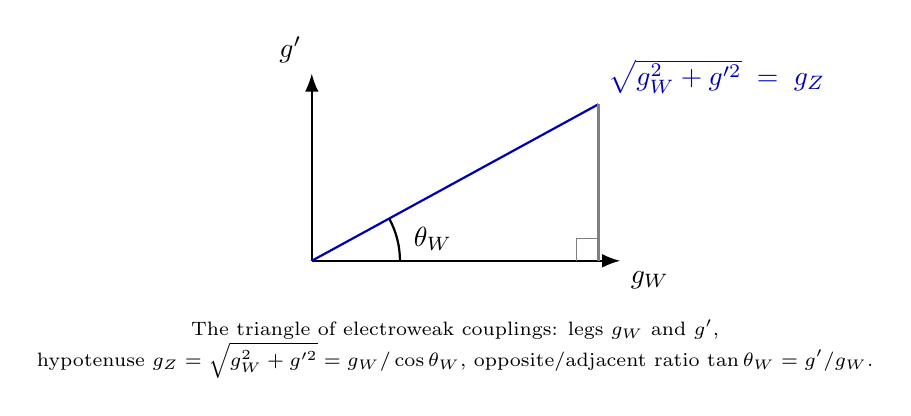
\begin{tikzpicture}[scale=2.8,>=Latex]
  \draw[->,thick] (0,0) -- (1.4,0) node[below right] {$g_W$};
  \draw[->,thick] (0,0) -- (0,0.85) node[above left]  {$g'$};
  \draw[thick,blue!70!black] (0,0) -- (1.3,0.71) node[above right] {$\sqrt{g_W^2 + g'^2}\;=\;g_Z$};
  \draw[thick,gray] (1.3,0) -- (1.3,0.71);
  \draw[gray] (1.20,0) -- (1.20,0.10) -- (1.30,0.10);
  \draw[thick] (0.4,0) arc (0:28.7:0.4);
  \node at (0.55,0.10) {$\theta_W$};
  \node[font=\scriptsize, align=center] at (0.65,-0.4)
    {The triangle of electroweak couplings: legs $g_W$ and $g'$,\\
     hypotenuse $g_Z = \sqrt{g_W^2 + g'^2} = g_W/\cos\theta_W$, opposite/adjacent ratio $\tan\theta_W = g'/g_W$.};
\end{tikzpicture}
\end{center}

\begin{intuitionbox}
\textbf{Why is this triangle useful?} It packages the three couplings $g_W$, $g'$, $g_e$ and
the angle $\theta_W$ into a single geometric object. Every fact you'd want to remember
about the electroweak couplings can be read off this triangle:
\begin{itemize}[leftmargin=*]
  \item $\tan\theta_W = g'/g_W$ (opposite over adjacent).
  \item $\sin\theta_W = g'/g_Z$, $\cos\theta_W = g_W/g_Z$ where $g_Z \equiv \sqrt{g_W^2 + g'^2}$.
  \item $g_e = g_W \sin\theta_W = g' \cos\theta_W$ (drop the perpendicular from the right
        angle to the hypotenuse; the foot of the perpendicular is at distance $g_e$ from
        the origin in the appropriate direction).
\end{itemize}
The hypotenuse $g_Z$ is the coupling of the $Z^0$ to fermions (modulo the $c_V, c_A$
factors --- see Griffiths Eq.~9.94 / Eq.~9.156).
\end{intuitionbox}

\subsection*{4.6 \,---\, The $Z^0$ coupling drops out as a bonus}

\begin{stepbox}[title=Step 4.6: Use the consistency relation to simplify the $Z$ piece]
Look at the $Z^\mu$ coefficient in Eq.~\eqref{eq:rotated}:
\[
\mathcal{L}_Z \;=\; -\,Z^\mu \!\left( g_W \cos\theta_W \, j^3_\mu \;-\; \tfrac{g'}{2} \sin\theta_W \, j^Y_\mu \right) .
\]
Use $g' = g_e/\cos\theta_W$ and $g_W = g_e/\sin\theta_W$ to eliminate $g_W$ and $g'$:
\begin{align}
\mathcal{L}_Z
&= -\,Z^\mu \!\left( \frac{g_e \cos\theta_W}{\sin\theta_W}\, j^3_\mu \;-\; \frac{g_e \sin\theta_W}{2 \cos\theta_W}\, j^Y_\mu \right) \notag\\[2pt]
&= -\,\frac{g_e}{\sin\theta_W \cos\theta_W}\, Z^\mu \!\left( \cos^2\theta_W\, j^3_\mu \;-\; \tfrac{1}{2} \sin^2\theta_W\, j^Y_\mu \right) \notag\\[2pt]
&= -\,\frac{g_e}{\sin\theta_W \cos\theta_W}\, Z^\mu \!\left( j^3_\mu \;-\; \sin^2\theta_W\, j^{\rm em}_\mu \right),
\label{eq:Zlag}
\end{align}
where in the last line I used $j^{\rm em} = j^3 + \tfrac{1}{2}j^Y$, so
$\cos^2\theta_W\, j^3 - \tfrac{1}{2}\sin^2\theta_W\, j^Y = j^3 - \sin^2\theta_W\,(j^3 + \tfrac{1}{2}j^Y) = j^3 - \sin^2\theta_W\, j^{\rm em}$.

Defining the $Z^0$ coupling
\[
g_Z \;\equiv\; \frac{g_e}{\sin\theta_W \cos\theta_W} \;=\; \sqrt{g_W^2 + g'^2}
\quad\text{(Griffiths Eq.~9.156)},
\]
\eqref{eq:Zlag} reads
\[
\mathcal{L}_Z \;=\; -\,g_Z\, Z^\mu \!\left( j^3_\mu - \sin^2\theta_W\, j^{\rm em}_\mu \right) .
\]
This is Griffiths Eq.~9.155. The structure $j^3 - \sin^2\theta_W\, j^{\rm em}$ is exactly what
generates the entries in Griffiths Table~9.1 (the famous $c_V$ and $c_A$ couplings of the
$Z^0$ to each fermion species).
\end{stepbox}

\subsection*{4.7 \,---\, Experimental value of $\theta_W$}

\begin{conceptbox}
The Weinberg angle is \emph{not} predicted by GWS; it must be measured. Modern global fits
to LEP, SLD, Tevatron, and LHC data give
\[
\sin^2\theta_W \;\approx\; 0.23146 \pm 0.00012
\quad\text{(Thomson Eq.~15.31; Mann Eq.~22.5)},
\]
which corresponds to $\theta_W \approx 28.75^\circ$. Griffiths quotes the same value (his
Eq.~9.95 / Eq.~10.95) to slightly less precision: $\sin^2\theta_W \approx 0.23$,
$\theta_W \approx 28.7^\circ$.
\end{conceptbox}

\begin{intuitionbox}
The fact that $\sin^2\theta_W$ is \emph{neither} 0 \emph{nor} 1 is what makes the
electroweak theory \emph{electroweak} --- the photon and the $Z$ are genuine \emph{mixtures}
of $W^3$ and $B$, not just one or the other:
\begin{itemize}[leftmargin=*]
  \item If $\theta_W = 0$: $\gamma = B$, $Z = W^3$. No mixing, two unrelated $U(1)$'s, no
        unification.
  \item If $\theta_W = 90^\circ$: $\gamma = W^3$, $Z = -B$. Photon would couple only to LH
        fields (parity-violating EM!) --- unphysical.
  \item Measured $\theta_W \approx 28.7^\circ$: photon is $\sim 77\%$ $B$ + $\sim 23\%$ $W^3$.
        The 23\% admixture of $W^3$ is what carries the (electromagnetic-like) coupling of the
        photon to charged \emph{left-handed} fermions through the weak isospin generator,
        completing the electroweak unification.
\end{itemize}
\end{intuitionbox}

\begin{resultbox}
\textbf{Part 4 result.}
\[
\boxed{\;
\tan\theta_W = \frac{g'}{g_W},
\qquad
g_W \sin\theta_W \,=\, g' \cos\theta_W \,=\, g_e,
\qquad
g_Z = \frac{g_e}{\sin\theta_W\cos\theta_W} = \sqrt{g_W^2 + g'^2}.
\;}
\]
The single parameter $\theta_W$ ties together \emph{three} couplings ($g_W, g', g_e$) and
\emph{four} gauge fields ($W^{1,2,3}, B \to W^\pm, Z, \gamma$). Experimental:
$\sin^2\theta_W \approx 0.231$.
\end{resultbox}

\newpage

% =====================================================================
% PART 5 — Why does the mixing happen?
% =====================================================================
\section*{Part 5 \,---\, \emph{Why} does the mixing happen? Higgs mechanism}

\begin{problembox}
\textbf{Restatement.} Conceptually: \emph{why} are $\{W^{1,2,3}, B\}$ \emph{not} themselves
the observed bosons? What dynamical mechanism forces the rotation? Explain the role of
the Higgs vacuum expectation value (VEV).
\end{problembox}

\begin{deliverbox}
Give a one-page conceptual explanation: the Higgs VEV spontaneously breaks
$SU(2)_L \otimes U(1)_Y \to U(1)_{\rm em}$, giving masses to three linear combinations of
the gauge fields ($W^\pm, Z$) and leaving one combination ($\gamma$) massless. Show how
diagonalizing the $(W^3, B)$ mass matrix reproduces the rotation of Part 3 and gives
$m_W = m_Z \cos\theta_W$.
\end{deliverbox}

\begin{strategybox}
There are two pictures of why the mixing happens:
\begin{itemize}[leftmargin=*]
  \item \textbf{Symmetry-counting picture:} $SU(2)_L \otimes U(1)_Y$ has 4 generators.
        $U(1)_{\rm em}$ has 1 generator. Therefore $4-1 = 3$ generators are ``broken'' by
        the Higgs VEV. By Goldstone's theorem, you'd get 3 massless Goldstone bosons; in a
        gauge theory they are ``eaten'' by 3 of the gauge fields, which become massive.
        The remaining 1 gauge field stays massless. That's the photon.
  \item \textbf{Mass-matrix picture:} Compute the gauge boson mass matrix from $|D_\mu \Phi|^2$
        evaluated at the Higgs VEV. The $(W^3, B)$ block is non-diagonal --- diagonalizing
        it gives \emph{exactly} the rotation we wrote down in Part 3, with
        $\tan\theta_W = g'/g_W$, and tells us $m_W = m_Z \cos\theta_W$ as a free bonus.
\end{itemize}
The mass-matrix picture is the more concrete one and gives explicit predictions, so we'll
sketch it here.
\end{strategybox}

\subsection*{5.1 \,---\, The Higgs doublet and its VEV}

\begin{conceptbox}
The Higgs scalar $\Phi$ is an $SU(2)_L$ doublet with hypercharge $Y_\Phi = +1$:
\[
\Phi(x) \;=\; \begin{pmatrix} \phi^+(x) \\ \phi^0(x) \end{pmatrix},
\qquad
\langle\Phi\rangle \;=\; \frac{1}{\sqrt{2}}\begin{pmatrix} 0 \\ v \end{pmatrix},
\qquad v \approx 246~\text{GeV}.
\]
The vacuum expectation value (VEV) $v$ is the value of the lower component at the minimum
of the Higgs potential $V(\Phi) = -\mu^2 \Phi^\dagger \Phi + \tfrac{\lambda}{2}(\Phi^\dagger \Phi)^2$
with $\mu^2 > 0$. Because the VEV picks out a specific direction in the $SU(2)_L$ doublet
space, it ``breaks'' the symmetry: the vacuum is not invariant under all of
$SU(2)_L \otimes U(1)_Y$ --- only under the subgroup that leaves $\langle\Phi\rangle$
invariant.

\textbf{Which subgroup leaves $\langle\Phi\rangle$ invariant?} A generator $X$ leaves the
vacuum invariant iff $X \langle\Phi\rangle = 0$. Plugging in $X = T^a$ ($a=1,2,3$) and
$X = Y/2$, you find that $T^1, T^2, (T^3 - Y/2)$ all act non-trivially on
$\langle\Phi\rangle$ (broken), while $(T^3 + Y/2) \langle\Phi\rangle = 0$ \emph{exactly}
because of the Gell-Mann--Nishijima formula $Q = T^{(3)} + Y/2$ and the fact that the lower
component of $\Phi$ has $T^{(3)} = -1/2, Y = +1$ giving $Q = 0$. So $Q$ generates the
unbroken subgroup, $U(1)_{\rm em}$. This is the photon's home.
\end{conceptbox}

\subsection*{5.2 \,---\, Compute the gauge field mass matrix}

\begin{stepbox}[title=Step 5.2: Plug $\langle\Phi\rangle$ into the kinetic term]
The Higgs kinetic term is $|D_\mu \Phi|^2$, with
\[
D_\mu \Phi \;=\; \!\left( \partial_\mu - i g_W\, T^a W^a_\mu - i \tfrac{g'}{2}\, Y_\Phi B_\mu \right)\!\Phi.
\]
At the VEV (replace $\Phi \to \langle\Phi\rangle$ and $\partial_\mu \to 0$):
\[
D_\mu \langle\Phi\rangle \;=\; -i\!\left( g_W\, T^a W^a_\mu + \tfrac{g'}{2}\, B_\mu \right)\!\langle\Phi\rangle .
\]
Computing $|D_\mu \langle\Phi\rangle|^2 = (D_\mu \langle\Phi\rangle)^\dagger (D^\mu \langle\Phi\rangle)$
and keeping the gauge-field bilinears, after some algebra one finds (Lancaster \& Blundell
Eq.~47.33, Mann Eq.~23.41-44):
\begin{equation}
|D_\mu \langle\Phi\rangle|^2
\;=\; \frac{v^2}{8} \!\left[ g_W^2 (W^1_\mu)^2 + g_W^2 (W^2_\mu)^2
        + (g_W W^3_\mu - g' B_\mu)^2 \right] .
\label{eq:HiggsMass}
\end{equation}
\end{stepbox}

\subsection*{5.3 \,---\, Read off the masses}

\begin{stepbox}[title=Step 5.3: Identify mass terms]
Recall the canonical mass term for a vector field is $\tfrac{1}{2} m^2 V_\mu V^\mu$.
Compare to \eqref{eq:HiggsMass}:
\begin{itemize}[leftmargin=*]
  \item \textbf{$W^1$ and $W^2$:} each gets a mass term $\tfrac{g_W^2 v^2}{8} (W^a_\mu)^2 = \tfrac{1}{2} \cdot \tfrac{g_W^2 v^2}{4} (W^a_\mu)^2$,
        giving $m_{W^1} = m_{W^2} = \tfrac{g_W v}{2}$. After the $W^\pm = \tfrac{1}{\sqrt2}(W^1 \pm i W^2)$
        rotation (Part 2), the same mass becomes
        \[
        \boxed{\;m_W \;=\; \tfrac{1}{2}\, g_W\, v.\;}
        \]
  \item \textbf{$(W^3, B)$ sector:} the term $(g_W W^3 - g' B)^2$ gives a $2\times 2$
        quadratic form in $(W^3, B)$. Expanding,
        \[
        (g_W W^3 - g' B)^2 \;=\; g_W^2 (W^3)^2 - 2 g_W g' W^3 B + g'^2 B^2 .
        \]
        Writing this as $\tfrac{1}{2} V_\mu^T M^2 V^\mu$ with $V = (W^3, B)^T$:
        \[
        M^2 \;=\; \frac{v^2}{4}
        \begin{pmatrix} \phantom{-}g_W^2 & -g_W g' \\[2pt] -g_W g' & \phantom{-}g'^2 \end{pmatrix} .
        \]
\end{itemize}
This mass matrix is \emph{not} diagonal --- the off-diagonal $-g_W g'$ entries are exactly
what \emph{forces} the rotation between $\{W^3, B\}$ and the mass eigenstates.
\end{stepbox}

\subsection*{5.4 \,---\, Diagonalize the $(W^3, B)$ mass matrix}

\begin{stepbox}[title=Step 5.4: Find eigenvalues and eigenvectors]
The mass matrix $M^2$ is rank-1 (its determinant is $g_W^2 g'^2 - g_W^2 g'^2 = 0$).
Therefore it has one zero eigenvalue and one non-zero eigenvalue.

\textbf{Trace gives the sum of eigenvalues:}
\[
\text{tr}(M^2) \;=\; \tfrac{v^2}{4}(g_W^2 + g'^2) \;=\; \lambda_+ + \lambda_- .
\]

\textbf{Determinant gives the product:}
\[
\det(M^2) \;=\; 0 \;=\; \lambda_+ \lambda_- \quad\Longrightarrow\quad \lambda_- = 0 .
\]
So
\[
\lambda_+ \;=\; \tfrac{v^2}{4}(g_W^2 + g'^2),
\qquad \lambda_- \;=\; 0 .
\]

\textbf{Eigenvector for $\lambda_- = 0$ (the photon):} solve
$M^2 \binom{a}{b} = 0$. The first row gives $g_W^2 a - g_W g' b = 0 \Rightarrow b = g_W a / g'$.
Normalizing $a^2 + b^2 = 1$:
\[
\binom{a}{b} \;=\; \frac{1}{\sqrt{g_W^2 + g'^2}} \binom{g'}{g_W}
\;=\; \binom{\sin\theta_W}{\cos\theta_W} ,
\]
using $\sin\theta_W = g'/\sqrt{g_W^2 + g'^2}$ and $\cos\theta_W = g_W/\sqrt{g_W^2 + g'^2}$.
So the massless eigenstate is
\[
A_\mu \;=\; W^3_\mu \sin\theta_W + B_\mu \cos\theta_W
\;\stackrel{!}{=}\; \text{Griffiths Eq.~9.151 photon definition.}\;\checkmark
\]

\textbf{Eigenvector for $\lambda_+$ (the $Z$):} the orthogonal direction:
\[
Z_\mu \;=\; W^3_\mu \cos\theta_W - B_\mu \sin\theta_W
\;\stackrel{!}{=}\; \text{Griffiths Eq.~9.151 $Z$ definition.}\;\checkmark
\]

\textbf{$Z$ mass:}
\[
\tfrac{1}{2} m_Z^2 \;=\; \lambda_+ \;=\; \tfrac{v^2}{4}(g_W^2 + g'^2)
\quad\Longrightarrow\quad
\boxed{\;m_Z \;=\; \tfrac{v}{2}\sqrt{g_W^2 + g'^2} \;=\; \frac{m_W}{\cos\theta_W} .\;}
\]
\end{stepbox}

\begin{insightbox}
\textbf{This is what ``the mixing happens'' actually means.} Diagonalizing the gauge boson
mass matrix \emph{is} the rotation of Part 3. The Weinberg angle is the diagonalization
angle of the $(W^3, B)$ mass matrix, which is in turn fixed by the ratio of the two gauge
couplings $g'/g_W$. The Higgs doesn't \emph{predict} $\theta_W$ --- the inputs $g_W, g'$
are still independent --- but it \emph{causes} the rotation by giving an off-diagonal mass
matrix.

The crucial fact is that the mass matrix has a \emph{zero} eigenvalue. This is not an
accident: it follows from the fact that the Higgs VEV is electrically neutral, so
$Q\langle\Phi\rangle = 0$, so the gauge field that couples to $Q$ stays massless. \textbf{The
photon is the gauge field of the unbroken subgroup} $U(1)_{\rm em}$, exactly as required
for QED to emerge at low energies.
\end{insightbox}

\subsection*{5.5 \,---\, $m_W = m_Z \cos\theta_W$: a precision-test prediction}

\begin{resultbox}
\textbf{From the diagonalization:}
\[
m_W \;=\; \tfrac{1}{2} g_W v,
\qquad
m_Z \;=\; \tfrac{v}{2}\sqrt{g_W^2 + g'^2} \;=\; \frac{m_W}{\cos\theta_W} .
\]
This gives the famous tree-level prediction
\[
\boxed{\; m_W \;=\; m_Z \cos\theta_W \;}
\quad\text{(Griffiths Eq.~9.98 / 10.98; Thomson §16.4).}
\]
With measured $m_Z = 91.188$ GeV and $\sin^2\theta_W \approx 0.231$ (so $\cos\theta_W \approx 0.877$),
this predicts $m_W^{\rm pred} \approx 79.94$ GeV, vs.\ measured $m_W = 80.385$ GeV. The
small discrepancy is one of the most precisely-tested radiative-correction predictions of
the Standard Model (top-quark and Higgs-mass loops; Thomson §16.4).
\end{resultbox}

\begin{intuitionbox}
\textbf{One-sentence summary of Part 5.} The Higgs vacuum is electrically neutral, so it
``feels'' the three broken generators $T^1, T^2, (T^3 - \tfrac{1}{2}Y)$ but \emph{not} the
unbroken combination $Q = T^{(3)} + \tfrac{1}{2} Y$. Three gauge fields couple to broken
generators and become massive ($W^\pm, Z$); the fourth, which couples to $Q$, stays massless
--- and \emph{that} is the photon.
\end{intuitionbox}

\newpage

% =====================================================================
% Final summary
% =====================================================================
\section*{Final Summary --- the answer to H2 in one box}

\begin{resultbox}
\textbf{Electroweak gauge group:} $SU(2)_L \otimes U(1)_Y$.

\textbf{Four ``fundamental'' gauge fields:}
\[
\underbrace{W^1_\mu,\; W^2_\mu,\; W^3_\mu}_{SU(2)_L\;\text{triplet,\;coupling}\;g_W}
\qquad\text{and}\qquad
\underbrace{B_\mu}_{U(1)_Y\;\text{singlet,\;coupling}\;g'}.
\]

\textbf{Four physical bosons (mass eigenstates):}
\[
\boxed{\;\;
\begin{aligned}
W^{\pm}_\mu &= \tfrac{1}{\sqrt{2}}\!\left( W^1_\mu \pm i\, W^2_\mu \right)
              & \text{(Griffiths Eq.~9.148)}, \\[3pt]
A_\mu       &= \phantom{-}B_\mu \cos\theta_W \;+\; W^3_\mu \sin\theta_W
              & \text{(Griffiths Eq.~9.151)}, \\[3pt]
Z_\mu       &= -B_\mu \sin\theta_W \;+\; W^3_\mu \cos\theta_W
              & \text{(Griffiths Eq.~9.151)}.
\end{aligned}
\;\;}
\]

\textbf{The Weinberg angle:}
\[
\tan\theta_W \;=\; \frac{g'}{g_W},
\qquad
g_W \sin\theta_W \;=\; g' \cos\theta_W \;=\; g_e
\quad\text{(Griffiths Eq.~9.154).}
\]

\textbf{Why the mixing:} the Higgs VEV $\langle\Phi\rangle = (0, v/\sqrt{2})^T$
spontaneously breaks $SU(2)_L \otimes U(1)_Y \to U(1)_{\rm em}$. The off-diagonal
$(W^3, B)$ mass matrix is diagonalized by exactly the $\theta_W$ rotation above. The
massless eigenstate is the photon; the orthogonal massive combination is the $Z^0$, with
$m_W = m_Z \cos\theta_W$.

\textbf{Experimental input:} $\sin^2\theta_W \approx 0.231$, so $\theta_W \approx 28.7^\circ$.
\end{resultbox}

\subsection*{Quick-reference one-line cheat sheet}

\noindent\fbox{\parbox{\linewidth}{\centering
$\;W^{\pm} = \tfrac{1}{\sqrt2}(W^1 \pm i W^2),
\quad
\binom{A}{Z} = \!\binom{\;\cos\theta_W \;\sin\theta_W\;}{\,-\sin\theta_W\;\cos\theta_W\,}\!\binom{B}{W^3},
\quad
\tan\theta_W = g'/g_W,
\quad
m_W = m_Z \cos\theta_W.$
}}

\end{document}
